% Contributions are much appreciated, in order to contribute to this project, head over to this repository:
% https://github.com/bshramin/uofa-eng-assignment

\documentclass[11pt,letterpaper]{article}
\textwidth 6.5in
\textheight 9.in
\oddsidemargin 0in
\headheight 0in
\usepackage{graphicx}
\usepackage{fancybox}
\usepackage[utf8]{inputenc}
\usepackage{epsfig,graphicx}
\usepackage{multicol,pst-plot}
\usepackage{pstricks}
\usepackage{amsmath}
\usepackage{amsfonts}
\usepackage{amssymb}
\usepackage{eucal}
\usepackage[left=2cm,right=2cm,top=2cm,bottom=2cm]{geometry}
\usepackage{esvect}
\pagestyle{empty}
\DeclareMathOperator{\tr}{Tr}
\newcommand*{\op}[1]{\check{\mathbf#1}}
\newcommand{\bra}[1]{\langle #1 |}
\newcommand{\ket}[1]{| #1 \rangle}
\newcommand{\braket}[2]{\langle #1 | #2 \rangle}
\newcommand{\mean}[1]{\langle #1 \rangle}
\newcommand{\opvec}[1]{\check{\vec #1}}
\renewcommand{\sp}[1]{$${\begin{split}#1\end{split}}$$}

\usepackage{lipsum}

\usepackage{listings}
\usepackage{color}
\usepackage{wrapfig}
\usepackage[shortlabels]{enumitem}

\definecolor{codegreen}{rgb}{0,0.6,0}
\definecolor{codegray}{rgb}{0.5,0.5,0.5}
\definecolor{codepurple}{rgb}{0.58,0,0.82}
\definecolor{backcolour}{rgb}{0.95,0.95,0.92}

\lstdefinestyle{mystyle}{
	backgroundcolor=\color{backcolour},   
	commentstyle=\color{codegreen},
	keywordstyle=\color{magenta},
	numberstyle=\tiny\color{codegray},
	stringstyle=\color{codepurple},
	basicstyle=\footnotesize,
	breakatwhitespace=false,         
	breaklines=true,                 
	captionpos=b,                    
	keepspaces=true,                 
	numbers=left,                    
	numbersep=5pt,                  
	showspaces=false,                
	showstringspaces=false,
	showtabs=false,                  
	tabsize=2
}

\lstset{style=mystyle}

\begin{document}
\pagestyle{plain}

\begin{flushleft}
Estudiante: Fabio Quimbay\\
Email: fabio.quimbay883@comunidadunir.net\\
Profesor: Miguel Ángel Cabeza\\
Fecha: Noviembre 4 de 2022\\
\end{flushleft}

\begin{flushright}\vspace{-20mm}

\includegraphics[height=2cm]{logo.png}
\end{flushright}
 
\begin{center}\vspace{0cm}
\textbf{\large PER5786 2022-2023  Física 1 (GFI) - PER5786 2022-2023}\\
 Tema 2 - Cinemática
\end{center}

 
\rule{\linewidth}{0.1mm}
%%%%%%%%%%%%%%%%%%%%%%%%%%%%%%%%%%%%%%%%%%%%%%%%%%%%%%%%%%%%%%%%%%%%%%%%

\bigskip
\bigskip

%%%%%%%%%%%%%%%%%%%%
\textbf{Ejercicio 3 propuesto}\\

La posición de una partícula que se mueve a lo largo del eje x varía con el tiempo t de acuerdo con la relación $x = t^3 - 12t + 20$, donde x se expresa en metros, y t en segundos.

\begin{enumerate}[(a)] 
\item {Encuentra la velocidad y la aceleración de la partícula en función del tiempo.}
\item {¿Ha habido alguna vez un momento en que $v = 0$?}
\item {Describe el movimiento de la partícula para $t \ge 0$}
\end{enumerate}

\textbf{Solución:}\\

\textbf{a)}: La derivada de la posición equivale a la velocidad y la derivada de la velocidad (doble derivada de la posición) equivale a la aceleración, a saber:

\begin{align}
	\vec{X}_{t} &= f(x) = t^3 - 12t + 20\\
	\vec{V}_{t} &= \frac{\partial f}{\partial t} = 3t^2 - 12\\
	\vec{A}_{t} &= \frac{\partial^2 f}{\partial t} = 6t
\end{align}

La velocidad y la aceleración en función del tiempo son $\vec{V}_{t}=3t^2 - 12$ y $\vec{A}_{t} = 6t$, respectivamente.\\

\textbf{b)}: Si ha habido un momento donde v = 0, a saber:

\begin{wrapfigure}{r}{0.25\textwidth}
    \centering
    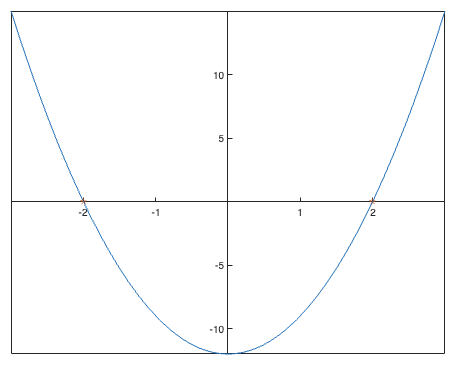
\includegraphics[width=0.25\textwidth]{ejemplo_3_punto_2.png}
\end{wrapfigure}

\begin{align*}
	\vec{V}_{t} &= 3t^2 - 12 = 0\\
	3t^2 &= 12\\
	t^2 &= \frac{12}{3} = 4\\
	\sqrt{t^2} &= \sqrt{4}\\
	t &= \pm 2
\end{align*}

La velocidad $\vec{V}_{t}=0$ cuando se tiene un $t = \pm 2$ seg.\\

\textbf{c)}: El movimiento de la partícula a partir de $t \ge 0$ esta descrito por la siguiente gráfica, a saber:

\begin{enumerate}[(a)] 
\item {La posición es decreciente, pero a partir del t=2.5s aprox. es creciente.}
\item {La velocidad esta descrita por un movimiento creciente.}
\item {La aceleración es lineal.}
\end{enumerate}

\begin{wrapfigure}{r}{0.35\textwidth}
    \centering
    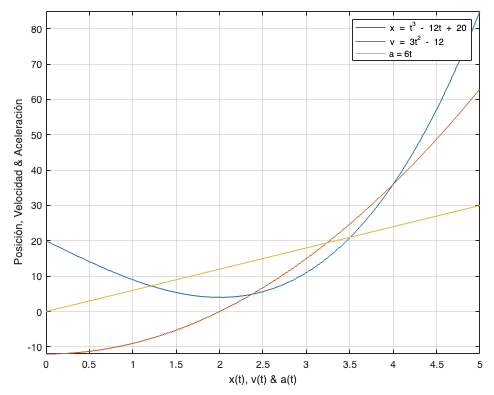
\includegraphics[width=0.35\textwidth]{ejemplo_3_punto_3.png}
\end{wrapfigure}

%%%%%%%%%%%%%%%%%%%%

\end{document}

